\begin{enunciado}{2}
    Show that for the learning model of positive rectangles (aligned horizontally or vertically), $m_{\hipotset}(4) = 2^4$ and $m_{\hipotset}(5) < 2^5$. Hence, give a bound for $m_{\hipotset}(N)$.
\end{enunciado}

Para mostrar que neste caso a $\dvc = 4$, nós precisamos mostrar duas coisas:

\textbf{1. Existem 4 pontos que podem ser estraçalhados}

A figura abaixo mostra como podemos separar 4 pontos utilizando retângulos.

\begin{figure}[h]
	\centering
	\begin{minipage}{0.46\textwidth}
		\centering
		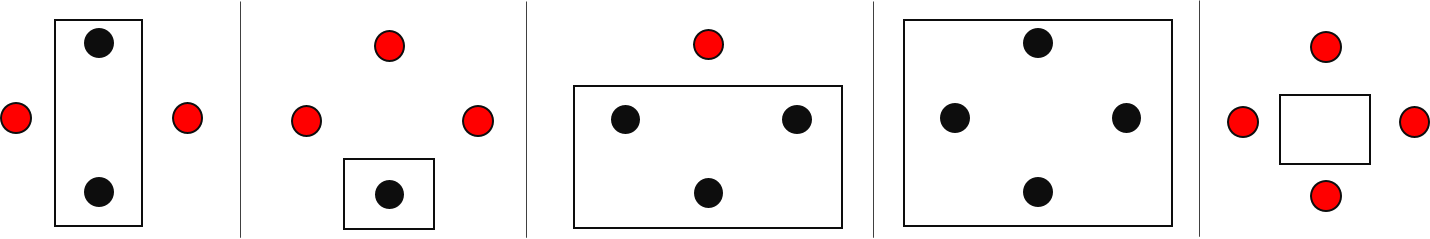
\includegraphics[width=\textwidth]{images/2-2-dvc4.png}
		\caption{Arranjo de 4 pontos que podem ser estraçalhados}
	\end{minipage}
\end{figure}

\textbf{2. Nenhum conjunto de 5 pontos pode ser estraçalhado}

Dados 5 pontos, uma combinação possível que pode ser estraçalhada deve nos permitir selecionar todos os 5 pontos
e, também, selecionar 4 pontos sem o quinto.

\begin{figure}[h]
	\centering
	\begin{minipage}{0.45\textwidth}
		\centering
		
\includegraphics[width=\textwidth]{images/2-2-dvc5.png}
		\caption{Arranjo de 5 pontos que não podem ser estraçalhados}
	\end{minipage}
\end{figure}

Logo, vê-se que o retângulo que nos permite selecionar todos os cinco pontos é definido por apenas quatro pontos
- um para cada aresta. Assim, é evidente que o quinto ponto deve situar-se quer por uma aresta ou no interior do
retângulo. Isso nos impede de selecionar quatro pontos sem o quinto, o que prova $\dvc < 5$.